\documentclass[../main.tex]{subfiles}
\graphicspath{{\subfix{../src/}}}


\begin{document}
\section{Problem Specification}

There is a large need for new technology that improves the effectiveness and ergonomics of human hand prosthetics.
Current state-of-the-art prosthetic products on the market exhibits a severe reduction of controllable degrees of Freedom compared to their biological counterparts.
Some prosthetics products are simple in design, often using a small set of motors to control multiple joints at the same time, furthermore, these products often rely on simple, grasp control based on 2 or more \gls{sEMG} interfaces.
These \gls{sEMG} interfaces are used to classify ``open/close'' signals generated by the muscles in the residual limb of the amputee.
The prosthetics user is manually required to change control-scheme between different grip typs, creating very crude control dynamics that is fundamentally different from biological hand control.
An example of a commercial prosthetic with this crude control design is the ``Ottobock Bebionic Hand EQD'' \cite{ottobock}.
The Ottobock hand is marketed as being a comfortable, intuitive \& adaptable prosthetic hand giving you natural and precise control of a vide range of grip types.
This is however far from the truth when reading the usage manual, that states that changing between grip types can be done by pressing a button on the top of the device for a second.
Furthermore, in order to move the thumb rotation joint, the user is asked to manually rack the thumb to the decired position.
None of these usage patterns provide meaningful and dynamic adaptability of the device, and is in no way intuitive compared to a real hand.
The Ottobock Ottobock Bebionic Hand EQD is priced at $\$30.000$ to $\$40.000$ \cite{ottobock-prices}.
The control pattern used in the Ottobock prosthetic hand follows the scheme shown in figure \ref{fig:nonidealprosthetic}.

\begin{figure}[H]
\begin{center}
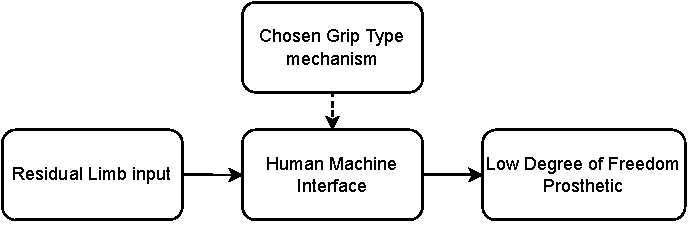
\includegraphics[width=0.8\textwidth]{NonIdealProsthetic.pdf}
\caption{Example of a commercial prosthetic hand's manual control scheme \cite{ottobock}.}
\label{fig:nonidealprosthetic}
\end{center}
\end{figure}

%TODO: I need examples to back up my slander of modern *commercial* prosthetics!
% Maybe explain they need to be like this to be robust, and that research methods are not robust enough yet to be commercial?

%A in-debth explanation of ``open/close'' control can be seen in section \ref{???}
%TODO: This sounds weird, integrate a simple controller therory here, and why it is so crude, then refrence it in state-of-the-art
%TODO: Create refrence
Crude controllability of upper-limb prosthetics is a great pitfall in the field of research and development of prosthetics, this has a large impact on rehabilitation of amputees.
The World Health Organization (WHO) defines rehabilitation as ``a set of interventions designed to optimize functioning and reduce disability in individuals with health conditions in interaction with their environment'' \cite{WHO_rehab}.
Proper rehabilitation and function of the prostetic is crucial to the independence of the amputee, but unsatisfactory function of prosthetics lead to amputees, that exhibit a great deal of stress during the rehabilitation process.
Insatisfaction and stress can cause the patient to repel the rehabilitation process and the prosthetic all-together \cite{Kristin2012}.
The repelling of the prostetic increase in the cases of the most severe cases of amputation, where the largest amount of control muscles are lost.
These amputations are often located further up the limbs, where the loss of mobility and controllability are greatest.
The type of prosthetic the amputee is able to recieve is highly dependent on the severity of the loss of limb, furthermore, the amount of muscles leftover from amputation also dicates the type of prosthetic interface the patient is able to interface with.
%TODO: Refrence for this!
Patients of hand amputation are able to recieve prosthetics with much more control of individual movements due to the muscles controlling the lost limb being intact. 
Lower-arm amputation patients has less control over their prosthetic due to the loss of the muscles in the lower-arm.
%TODO: Tech2015 can be a good ref for state-of-the-art stuff 
The differences between severity is a problem in prosthetics design because it is impossible to create a standardized prosthetic that suits most patient's needs.

%TODO: This one is bad
%State-of-the-art commercial prosthetics further decrease the controllable DoF in order to increase robustness of the control experience, this is further elaborated upon in \ref{sec:stateoftheart}.
%TODO: Create refrence for state-of-the-art

%TODO: Problem specification should be an entire page!
% \newpage
\subsection{Motivation}

The main goal of this thesis is to provide a meaningful contribution to the world of prosthetics design and control.
Modern state-of-the-art commercial prosthetic hands are in no way compareable to their real life counterparts.
The ideal control scheme of a prosthetic device is the control-scheme used by a real human hand, this control scheme can be seen in figure \ref{fig:idealprosthetic}.

\begin{figure}[h]
\begin{center}
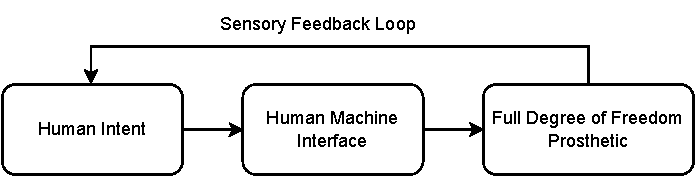
\includegraphics[width=0.8\textwidth]{IdealProsthetic.pdf}
\caption{The Ideal design of a prosthetic hand, that mimics the chontrol scheme of a real hand.}
\label{fig:idealprosthetic}
\end{center}
\end{figure}

%TODO: This is not good, because i dont go into detail with this in my thesis..
% One of the important features of the hand, often neglected by commercial products is the hand's usage as a sensory device, and that the control of a hand is closely related to a closed-loop between the user's intent and the hand's actions that in turn create sensory feedback to the user.

This thesis aims to contribute to the world of prosthetics control, and by doing so, research methods of bringing current state-of-the-art prosthetics closer to their real life counterparts.
This gap exists in terms of controllability and dynamic modification of grip types, and will be focused on by researching effective methods of collecting sensory data from the lower-/upper-arm.
By researching effective data collection methods, it is hoped that the contribution of the thesis would be shifting modern methods closer to an adaptive controller that is able to imitate the intent and movements or a real hand.
%This thesis aims to summarize, and compare current state-of-the-art prosthetics research and products, and products the control of prosthetics and the existing limitations of these state-of-the-art products. 
Increasing the controllability of a prosthetic, by improving data collection and interpretation of  sEMG signals, will provide a more true-to-life experience to the prosthetics user, and thus reduce the amount of patients that disregard prosthetics, and increase overall amputee independence.
Lastly, this thesis aims to design a simulated, anatomically correct prosthetic hand with the purpose of testing the developed methods.


\newpage
\subsection{Goals}
\label{sec:goals}

In order to define the reserach and development of this thesis, a set of development goals has been made:

%TODO: Refer to these in the report! make it the key motivations for all my choises.
\begin{enumerate}
\item Create a software-based, biology-inspired, anatomically realistic simulation of a humanoid lower-arm/hand that is able to imitate the movements of the human hand.
\item Create a dynamic software interface to control the software-based prosthetic hand using a widely-used robotics communication interface.
\item Reserach and design sEMG based pre-prossesing pipelines for a prosthetics controller, with the purpose of eliminating noise and increasing meaningful aspects as input to a controller. 
\item Research and design state-of-the-art prosthetics controllers based on machine learning and artificial intelligence, with the focus of increasing overall controllability and adaptability of a simulated prosthetic hand.
\item Design a set of core day-to-day movement types of the hand, that can be reproduced by 1 or more prople in order to create a dataset applicable to train the designed controller models.
\item Test and Validate the created controller models on the simulated prosthetic hand, in order to assess the applicability of the designed methods.
\end{enumerate}

\end{document}
